\documentclass[final,hyperref={pdfpagelabels=false}]{beamer}
\usepackage{grffile}
\usepackage{ragged2e}
\mode<presentation>{\usetheme{I6pd2}}
\usepackage[english]{babel}
\usepackage[latin1]{inputenc}
\usepackage{amsmath,amsthm, amssymb, latexsym}
 \usepackage{setspace}
 \linespread{0.6}
\setbeamertemplate{bibliography item}[text] 
%\usepackage{times}\usefonttheme{professionalfonts}  % obsolete
%\usefonttheme[onlymath]{serif}
\boldmath
\usepackage[orientation=portrait,size=a0,scale=0.95,debug]{beamerposter}
\usepackage{graphicx}
\setbeamertemplate{caption}[numbered]
% change list indention level
% \setdefaultleftmargin{3em}{}{}{}{}{}


%\usepackage{snapshot} % will write a .dep file with all dependencies, allows for easy bundling

\usepackage{array,booktabs,tabularx}
\newcolumntype{Z}{>{\centering\arraybackslash}X} % centered tabularx columns
\newcommand{\pphantom}{\textcolor{ta3aluminium}} % phantom introduces a vertical space in p formatted table columns??!!

\listfiles

%%%%%%%%%%%%%%%%%%%%%%%%%%%%%%%%%%%%%%%%%%%%%%%%%%%%%%%%%%%%%%%%%%%%%%%%%%%%%%%%%%%%%%
\graphicspath{{figures/}}
 
\title{\huge Effects of noise gene expression on background and cooperation-defector fitness}
\author{Luis Alejandro Mahecha and Juan Manuel Pedraza}
\institute[Universidad de los Andes]{Department of Physics, Universidad de los Andes, Bogota, Colombia \\  Facultad de Ciencias Proyecto Semilla}
\date[Sep. 8th, 2009]{Sep. 8th, 2009}

%%%%%%%%%%%%%%%%%%%%%%%%%%%%%%%%%%%%%%%%%%%%%%%%%%%%%%%%%%%%%%%%%%%%%%%%%%%%%%%%%%%%%%
\newlength{\columnheight}
\setlength{\columnheight}{100cm}


%%%%%%%%%%%%%%%%%%%%%%%%%%%%%%%%%%%%%%%%%%%%%%%%%%%%%%%%%%%%%%%%%%%%%%%%%%%%%%%%%%%%%%
\begin{document}
\begin{frame}
  \begin{columns}
    % ---------------------------------------------------------%
    % Set up a column 
    \begin{column}{.49\textwidth}
      \begin{beamercolorbox}[center,wd=\textwidth]{postercolumn}
        \begin{minipage}[T]{.95\textwidth}  % tweaks the width, makes a new \textwidth
          \parbox[t][\columnheight]{\textwidth}{ % must be some better way to set the the height, width and textwidth simultaneously
            % Since all columns are the same length, it is all nice and tidy.  You have to get the height empirically
            % ---------------------------------------------------------%
            % fill each column with content            
            \begin{block}{Abstrac}
\justifying \small The models of evolutionary dynamics are usually based in a fixed background fitness, and when they include cooperation, they also include a fixed degree of cooperation. However, in a biological system each individual is going to have different fitness and cooperate in different degrees due to phenotypic variability, even in isogenic populations.This is an effect of the gene expression noise. Expression noise affects the fitness of an organism when its fitness depends on the advantage of some phenotype that is generate by a gene or group of genes, and an increase in gene noise expression can lead to a decrement of the average total fitness.\vskip+1.5ex
We firs set up an stochastic program for individual and group selection with fixed background fitness and cooperation. Then we introduced phenotype variability in the case of individual selection and finally we adapted the simulation to a common good game with group selection.\vskip+1.5ex  
 Our stochastic simulations show that the fixation time is altered if the background fitness is a non-linear function of the gene expression. Including phenotypic variability in Moran processes allows a more realistic approach to the evolution of
cooperation. Detailed simulations of competition populations of cooperators and defectors would allow characterization of the importance of phenotypic variability and its utility or impact as an evolutionary strategy.       
\end{block}

\begin{block}{Evolution and Fitness}
\justifying In evolution and organism with a certain characteristic can evolve  a new characteristic. When the old and new characteristic compete, the new is going to fixate in the population if it represents a better fitness for the organism Figure 1. This small scale evolution process changes the gene or allele frequency in a population from one generation to next\footnote{\url{ http://evolution.berkeley.edu/evolibrary/article/0_0_0/evo_02}}.
%\begin{column}{.25\paperwidth}
  %\vskip8ex
  \begin{figure}
        \begin{center}
  \includegraphics[width=11cm,height=8cm]{images/evolution.pdf}
     \end{center}
      \caption{fixation of a new type(red ball) in the old population(blue balls)} 
   \end{figure}
  Fitness is usually defined as the reproduction rate of each individual, and it can be due to a phenotype (in our case, background fitness) or behavior (in our case, to cooperate or defect). \vskip+1.5ex

The probability of being selected for reproduction for one type of  individual is proportional to its fitness, which may depend on its frequency. When individuals grow as a group, this process of natural selection can be happen in two levels, not just selecting the fittest individuals within a group, but also selecting the fittest groups.\cite{Traulsen2005}. Therefore the different types of fitness and levels of selection  are important to understand the dynamics of evolutionary processes.\vskip+1.5ex
\textbf{ Moran process}\\
The process of competition between two types is simulated as a Monte Carlo program using the Moran process algorithm. At each time step a type in a population of size $N$ is selected for reproduction with a probability $P_{A}$ proportional to its fitness $f_{A}$ and frequency $i$, and a random individual is replaced by the offspring (Figure 2). 
     %   \vskip2ex
      %\end{column}   
  \begin{tabularx}{\linewidth}{ZZ}     
   \begin{figure}
        \begin{center}
  \includegraphics[width=11cm,height=8cm]{images/Moranprocess.pdf}
     \end{center}
      \caption{Moran process with two types of genes A(red balls) and B(blue balls).} 
   \end{figure}
   &
   \begin{equation}
   P_{A}=\frac{if_{A}}{if_{A}+(N-i)f_{B}}
   \end{equation}
     \begin{equation}
   {P_{A}}(i ,i+1)=\frac{if_{A}}{if_{A}+(N-i)f_{B}}\frac{N-i}{N}
   \end{equation}
   \\
   \end{tabularx}
   To simulate group selection we consider a population of $m$ and groups with a maximum size of $n$ individuals with interactions only among the members of the same group. Individuals within a group reproduce  until it reaches size $n$, when it divides with probability $q$, which is much smaller than the individual reproduction rate.
   \vskip+1.5ex
With the Moran algorithm we simulate the probability of fixation for one group and group selection, using deterministic fitness, Figures 3 and 4.

\begin{tabularx}{\linewidth}{ZZ}
\begin{figure}
\includegraphics[width=11cm,height=8cm]{images/plot.pdf}
\caption{\textbf{Individual selection:} Probability of fixation of $50$ mutants as a function of their background fitness in a group of size $100$, with background fitness of $s=1$ for the other type.}
\end{figure}
&
\begin{figure}
\includegraphics[width=11cm,height=8cm]{images/m10n10q0001.pdf}
\caption{\textbf{Group selection:} Probability of fixation of a single mutant as a function of its fitness. The population has $10$ groups of size $10$, the splitting probability is $q=0.001$ and the other type has fitness $s=1$}
\end{figure}
\\
\end{tabularx}
\end{block}

\begin{block}{No deterministic fitness due to internal gene expression noise}
\justifying Fitness in an organism is not deterministic because it is affected by the internal gene expression noise \cite{Wang2011}. This intrinsic noise producess the differences among a group of isogenic cell in an homogenous medium,  leading to a fitness distribution for an allele (Figure  5). Therefore fitness is a function of gene expression,  and it has optimal values, because if the expression is too high the organism is wasting energy. This means that fitness is not a linear function of expression (Figure  6). \vskip+1.5ex
The probabilities for type $A$ of being selected for reproduction and increasing its frequency by 1 are  
\begin{equation}
P_{A}=\frac{\sum_{j=1}^{i}f_{Aj}}{\sum_{j=1}^{i}f_{Aj} + \sum_{j=1}^{N-i}f_{Bj}} \;\;\; P_{A}(i,i+1)=\frac{\sum_{j=1}^{i}f_{Aj}}{\sum_{j=1}^{i}f_{Aj} + \sum_{j=1}^{N-i}f_{Bj}}\frac{N-i}{N}.
\end{equation}

In our simulation we measure the effects of noise on the average fixation time of an allele in a constant population size. We  used a gaussian protein distribution with varying mean and noise (Figure 7).
                 %\begin{column}{.44\textwidth}\centering
\begin{tabularx}{\linewidth}{ZZZ}
\begin{figure}
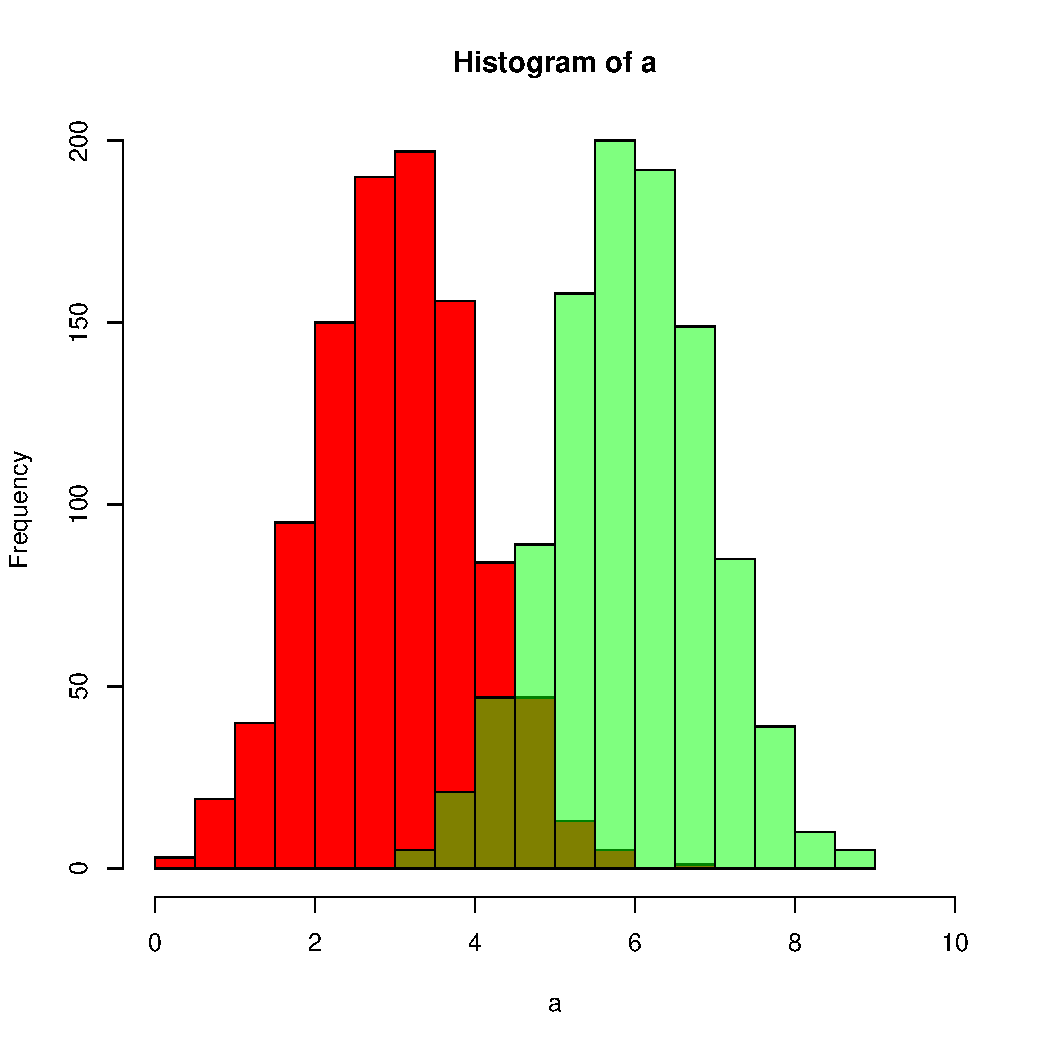
\includegraphics[width=11cm,height=8cm]{images/Rplots.pdf}
\caption{Gaussians distributions of proteins or degrees of cooperation for two different alleles.}
\end{figure}
&
\begin{figure}
\includegraphics[width=11cm,height=8cm]{images/TriangularFunction.jpg}
\caption{Fitness triangular function.}
\end{figure}
&
\begin{figure}
\includegraphics[width=11cm,height=8cm]{images/triangularfunctionHistogram.pdf}
\caption{Distribution of fitness generated by the triangular function.}
\end{figure}
\\
\end{tabularx}
\begin{tabularx}{\linewidth}{ZZZ}
\begin{figure}
\includegraphics[width=11cm,height=8cm]{images/SigmaVariationLTfitness.pdf}
\caption{Average time when $10$ initial mutants(mean fitness=2) reach  $50\%$ of the population. This graph shows the average  time using a gaussian distribution with a linear function and with a non-linear function centered with the gaussian distribution. }
\end{figure}
&
\begin{figure}
\includegraphics[width=11cm,height=8cm]{images/nocenteredVsSigma.pdf}
\caption{Average fixation time when the expression distribution is not centered with the fitness function. Fitness function centered on $10$ and distribution centered on $11$ and $12$.}
\end{figure}
&
\begin{figure}
\includegraphics[width=11cm,height=8cm]{images/AveragetimeFitness.pdf}
\caption{Average fixation time as a function of the mean fitness.}
\end{figure}
\\
\end{tabularx}
               % \end{colum
\end{block}
\vfill                     
          }
        \end{minipage}
      \end{beamercolorbox}
    \end{column}
    % ---------------------------------------------------------%
    % end the column

    % ---------------------------------------------------------%
    % Set up a column 
    \begin{column}{.49\textwidth}
      \begin{beamercolorbox}[center,wd=\textwidth]{postercolumn}
        \begin{minipage}[T]{.95\textwidth} % tweaks the width, makes a new \textwidth
          \parbox[t][\columnheight]{\textwidth}{ % must be some better way to set the the height, width and textwidth simultaneously
            % Since all columns are the same length, it is all nice and tidy.  You have to get the height empirically
            % ---------------------------------------------------------%
            % fill each column with content
            \begin{block}{Fitness due to altruistic behavior}
            Fitness due to cooperation is proportional to the utility of the altruistic act. The payoffs of cooperator-defector interactions are in the following  payoff matrices\cite{Traulsen2006a,Nowak2011}. 
            \begin{equation}
\bordermatrix{~ & C & D \cr
             C & b-c & -c \cr
              D & b & 0 \cr} \;\;\; or\;generally \;\;\; 
\bordermatrix{~ & C & D \cr
             C & R & S \cr
              D & T & P \cr} 
\end{equation}
The expected payoff $\pi_{C}$ of cooperators due to pairwise encounters with the rest of individuals in the group, and its fitness $f_{C}$ are:
\begin{equation}
 \pi_{C}=\frac{R(i-1)+S(n-i)}{n-1} \;\;\;\;\; f_{C}=1-w+w\pi_{C}.
\end{equation}
 $w$ is the intensity of selection, reflacting how much the interaction contributes to the fitness, and $1$ is the background fitness for random drift.
           
\begin{tabularx}{\linewidth}{ZZ}
\begin{figure}
\begin{center}
  \includegraphics[width=11cm,height=8cm]{images/groupselection.pdf}
     \end{center}
    \caption{Competition between cooperators and defectors in group selection. Where $q=0.001$ and $w=1$. The peaks are the splitting of a group.} 
   \end{figure}
&
\begin{figure}
        \begin{center}
  \includegraphics[width=11cm,height=8cm]{images/cirticbc.pdf}
     \end{center}
      \caption{Benefit to cost ratio. The point where one cooperator or defector has the same probability to take the whole population as a function of the number $m$ of groups with $n=10$. } 
   \end{figure}
   \\
\end{tabularx}
 \end{block}
            %\vfill
\begin{block}{Stochastic Cooperation}
              \justifying {\footnotesize  In this model  each individual invests a random cost $c_{i}$, and everyone obtains a common benefit $b=B\frac{\sum c_{i}}{n}$, where the benefit factor $B\geqslant1$ . The utility of each individual is $u_{i}=b-c_{i}$. Therefore, if everyone cooperates with the same amount they get back a larger amount, but if just some individuals cooperate, they will get back a smaller amount than invested. Furthermore, if nobody cooperate, there will be not payoff. } 
            \begin{figure}
        \begin{center}
  \includegraphics[width=11cm,height=8cm]{images/commongoodCooperation.pdf}
     \end{center}
      \caption{Individuals pay a cost $c_{i}$ and get back a common benefit $b$.} 
   \end{figure}
   The expected payoff of a cooperator is
   \begin{equation}
   \pi_{C}=\frac{\sum_{j=1}^{i}b-c_{cj}}{i}
   \end{equation}   
   and the fitness is
   \begin{equation}
   f_{c}=1-w+w\pi_{c}
   \end{equation} 
   In our simulations we used $w=1$.\vskip+1.5ex
 This describes a classic game in behavioral economics\cite{Szabo2002} where a  group of people is given an amount of money, each person has to contribute money, and the total amount is divided by the number of people in the group, and then each individual gets back this quantity times a factor larger than one.\vskip+1.5ex
    In a bacterial example, plasmids in E.coli are the individuals and the E.coli are the groups. The plasmids take nutrients from the cell for their own reproduction, but when they take too much the bacteria will reproduce slower. \vskip+1.5ex
    
 \justifying We used this cooperation model to simulate group selection in individuals with no deterministic degree  of cooperation. The population was divided in two types, where their cooperation degrees come from Gaussian distributions with different means and standard deviations as shown in (Figure 5). 
  
                 
                  \begin{tabularx}{\linewidth}{ZZ}
                  \begin{figure}
                   \includegraphics[width=11cm,height=8cm]{images/fixprobabilityVsmean0.pdf}
                   \caption{Fixation probability of cooperators as a function mean degree of defectors cooperation.}
                   \end{figure}
                  
                    &
                    \begin{figure}
                     \includegraphics[width=11cm,height=8cm]{images/fixprobabilityVsmean1Benefit.pdf}
                     \caption{Fixation probability of cooperators as a function of their mean degree cost. The shows different points for different values of benefit when all the groups are initially homogenous.}
                    \end{figure}
                    \\
                                    
                       \begin{figure}
                     \includegraphics[width=11cm,height=8cm]{images/probaCoopeSinglegroup.pdf}
                     \caption{Fixation probability of $50$ cooperators in a group of size $100$.}
                     \end{figure}

                     &
                       \begin{figure}
                     \includegraphics[width=11cm,height=8cm]{images/probaCoomixedGroup.pdf}
                     \caption{Fixation probability when a population of $m=10$ and $n=10$ has initially a mixed group with $5$ cooperators and the rest of the groups are deffectors.}
                     \end{figure}
                       \\
                   \end{tabularx}

             \end{block}
                        \begin{block}{Conclusions}
              \begin{itemize}
             \item The mean time of fixation is not affected if fitness is a linear function of protein expression.
             \item The mean fixation time is affected when the fitness is not a linear function of protein expression, and it is longer when genetic noise is larger. But if we see the distribution fitness that result from the fitness function, the mean fitness determines the average time fixation. This means that the fitness standard deviation dose not affect.
             \item  In group selection when all the initial groups are homogeneous, the fixation of probability dose not depend on the benefit(Figure 15), but as it is seen in (Figure 17) when there is an initial mixed group fixation probability is affected by benefit. 
             \item  In (Figure16) is observed the first level of cooperation, where cooperator are fitter as the benefit increase. From Figures (16 and 17) is observed that the two levels of selection have different behavior  as a function of benefit.         
              \end{itemize}
            \end{block}
            \begin{block}{References}
            {\small 
      % \setbeamertemplate{bibliography item}[text] 
       \bibliographystyle{plain} 
       \bibliography{poster}    % i.e. the poster.bib file 
     } 
            \end{block}
          }
          % ---------------------------------------------------------%
          % end the column
        \end{minipage}
      \end{beamercolorbox}
    \end{column}
    % ---------------------------------------------------------%
    % end the column
  \end{columns}
  \vskip1ex
  %\tiny\hfill\textcolor{ta2gray}{Created with \LaTeX \texttt{beamerposter}  \url{http://www-i6.informatik.rwth-aachen.de/~dreuw/latexbeamerposter.php}}
% \tiny\hfill{Created with \LaTeX \texttt{beamerposter}  \url{http://www-i6.informatik.rwth-aachen.de/~dreuw/latexbeamerposter.php} \hskip1em}
\end{frame}
\end{document}


%%%%%%%%%%%%%%%%%%%%%%%%%%%%%%%%%%%%%%%%%%%%%%%%%%%%%%%%%%%%%%%%%%%%%%%%%%%%%%%%%%%%%%%%%%%%%%%%%%%%
%%% Local Variables: 
%%% mode: latex
%%% TeX-PDF-mode: t
%%% End:
